

%\documentclass[12pt]{article}
\documentclass[12pt]{scrartcl}
\title{ELEC 340 Assignment 3}
\nonstopmode
%\usepackage[utf-8]{inputenc}
\usepackage{graphicx} % Required for including pictures
\usepackage[figurename=Figure]{caption}
\usepackage{float}    % For tables and other floats
\usepackage{verbatim} % For comments and other
\usepackage{amsmath}  % For math
\usepackage{amssymb}  % For more math
\usepackage{enumitem}
\usepackage{fullpage} % Set margins and place page numbers at bottom center
\usepackage{paralist} % paragraph spacing
\usepackage{listings} % For source code
\usepackage{subfig}   % For subfigures
%\usepackage{physics}  % for simplified dv, and 
\usepackage{enumitem} % useful for itemization
\usepackage{siunitx}  % standardization of si units

\usepackage{tikz,bm} % Useful for drawing plots
%\usepackage{tikz-3dplot}
\usepackage{circuitikz}
\usepackage{ctable}
\usepackage{multicol}
%%% Colours used in field vectors and propagation direction
\definecolor{mycolor}{rgb}{1,0.2,0.3}
\definecolor{brightgreen}{rgb}{0.4, 1.0, 0.0}
\definecolor{britishracinggreen}{rgb}{0.0, 0.26, 0.15}
\definecolor{cadmiumgreen}{rgb}{0.0, 0.42, 0.24}
\definecolor{ceruleanblue}{rgb}{0.16, 0.32, 0.75}
\definecolor{darkelectricblue}{rgb}{0.33, 0.41, 0.47}
\definecolor{darkpowderblue}{rgb}{0.0, 0.2, 0.6}
\definecolor{darktangerine}{rgb}{1.0, 0.66, 0.07}
\definecolor{emerald}{rgb}{0.31, 0.78, 0.47}
\definecolor{palatinatepurple}{rgb}{0.41, 0.16, 0.38}
\definecolor{pastelviolet}{rgb}{0.8, 0.6, 0.79}


\begin{document}

\begin{center}
\specialrule{0.02em}{}{}
\hrule
\vspace{0.3cm}
	{\textbf { \large {Discrete Structures (MA5.101) }}} 
\end{center}
\textbf{Instructor:}\ Dr. Ashok Kumar Das \hspace{\fill}\textbf{Assignment 3 Solutions}    \\
{\textbf{IIIT Hyderabad}   } \hspace{\fill} \textbf{Total Marks}: 70 \\ 
% keep it at the left side
\specialrule{0.01em}{}{}
\hrule

\paragraph*{Problem 1 } 

\\ Will be uploaded later by me[Jai] .

\paragraph*{Problem 2 }

\\ Will be uploaded later by me[Jai] .

\paragraph*{Problem 3 }
\\ Will be uploaded later by me[Jai] .

\paragraph*{Problem 4}
\\ Will be uploaded later by me[Jai] .

\paragraph*{Problem 5}
Say if $\mathbb{P}$ denotes the set of irrational numbers. $\mathbb{R} = \mathbb{Q} \cup \mathbb{P}$ and $\mathbb{P} \cap \mathbb{Q} = \phi$. We have the function as -
\begin{align*}
    f(x) &= \begin{cases}
    x , \text{ when }x \in \mathbb{Q} \\
    1 - x,  \text{ when } x \in \mathbb{P}
    \end{cases}
\end{align*}
To prove it is invertible, we need to prove that it is bijective. 
\begin{enumerate}
    \item \textbf{For one-one}.
    \\ We need to prove
    \begin{align*}
        f(x_1) = f(x_2) \implies x_1 = x_2
    \end{align*}
    Now we have 2 cases here - 
    \begin{enumerate}[a.]
        \item 
        \begin{align*}
            & f(x_1)  \in \mathbb{Q}, f(x_2) \in \mathbb{Q}
        \end{align*}
        Thus we have from our definition -
        \begin{align*}            
             & f(x_1) = f(x_2)
            \\ &\implies x_1 = x_2
        \end{align*}
        Thus $f(x_1) = f(x_2) \implies x_1 = x_2$.
        as if $1 - x_2$ is irrational, then $x_2$ is irrational. Since $\mathbb{Q} \cap \mathbb{P} = \phi$, we have $x_1 \neq x_2$.
        \item 
        \begin{align*}
            & f(x_1)  \in \mathbb{P}, f(x_2) \in \mathbb{P}
        \end{align*}
        Thus we have from our definition -
        \begin{align*}            
             & f(x_1) = f(x_2)
             \\ &\implies 1 - x_1 = 1 - x_2
            \\ &\implies x_1 = x_2
        \end{align*}
        Thus $f(x_1) = f(x_2) \implies x_1 = x_2$.
        as if $1 - x_2$ is irrational, then $x_2$ is irrational. Similarly for $x_1$.
    \end{enumerate}
    If we assume $f(x_1) = f(x_2)$ , since $\mathbb{Q} \cap \mathbb{P} = \phi$, we can never have
        \begin{align*}
            & f(x_1)  \in \mathbb{P}, f(x_2) \in \mathbb{Q}
        \end{align*}
    or 
        \begin{align*}
            & f(x_1)  \in \mathbb{Q}, f(x_2) \in \mathbb{P}
        \end{align*}
        \item \textbf{For onto}
        \\ We need to prove 
        \begin{align*}
            \forall y \in \mathbb{R}, \exists x \in \mathbb{R} \text{ such that } f(x) = y
        \end{align*}
        We have 2 cases -
        \begin{enumerate}[a.]
            \item 
            \begin{align*}
                y & \in \mathbb{Q}
            \end{align*}
            Take $x = y$, we have 
            \begin{align*}
                f(x) &= x = y
            \end{align*}
            \item 
            \begin{align*}
                y & \in \mathbb{P}
            \end{align*}
            Take $x = 1 - y$, since $y \in \mathbb{P}$, we have $x \in \mathbb{P}$. By definition, we have 
            \begin{align*}
                f(x) &= (1 - (1 - y)) = y
            \end{align*}            
        \end{enumerate}
\end{enumerate}
Construct $f^{-1}$ as - 
\begin{align*}
    f^{-1}(y) &= \begin{cases}
    y , \text{ when }y \in \mathbb{Q} \\
    1 - y,  \text{ when } y \in \mathbb{P}
    \end{cases}
\end{align*}
Proof that it is inverse [not necessary] - 
\begin{enumerate}
    \item \begin{align*}
        x &\in \mathbb{Q}
        \\ & f^{-1}(f(x)) 
        \\ &= f^{-1}(x) 
        \\ &= x
    \end{align*}
    \item \begin{align*}
        x &\in \mathbb{P}
        \\ & f^{-1}(f(x)) 
        \\ &= f^{-1}(1 - x) 
        \\ &= 1 - (1 - x)
        \\ &= x
    \end{align*}    
\end{enumerate}
We have 4 marks each for the one-one and onto, and 2 marks for the construction.

\paragraph*{Problem 6}
There are 3 ways to do it. All of them follow the structure below -
\begin{enumerate}
    \item State the bijection (mathematically or geometrically). [4 marks]
    \item Prove that it is a bijection. [4 marks]
    \item Mention the points on sphere (or plane) which are left unmapped and how you would deal with them. [2 marks]
\end{enumerate}
\textbf{Method 1:}
\\ \textbf{Stereographic Projection -} 
\begin{center}
    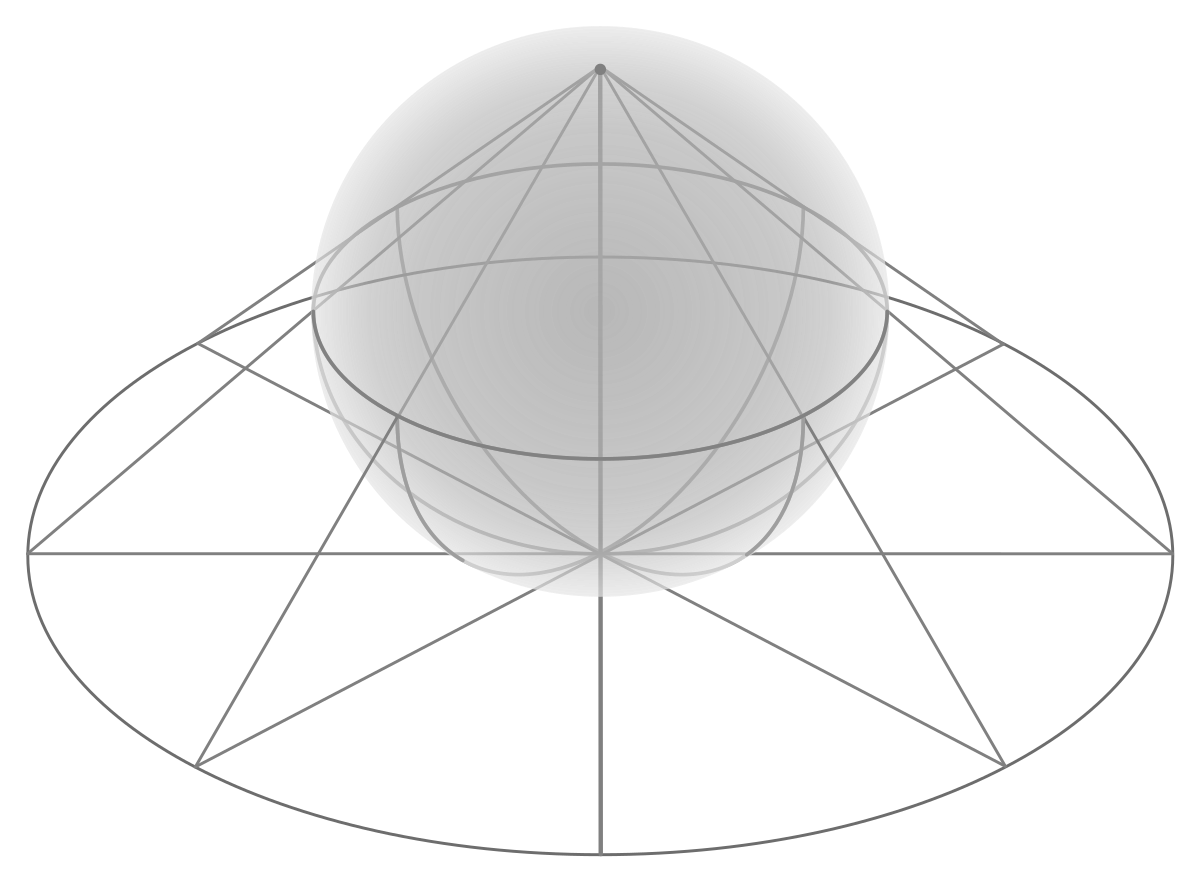
\includegraphics[width=0.5\linewidth]{1200px-Stereographic_projection_in_3D.svg.png}
\end{center}
Take a unit sphere. Let $P = (0,0,1)$ be the point of projection. Let $A$ and $B$ be the set of points on the sphere and Construct an $f:{A - \{P\}} \rightarrow {B}$ such that, 
\begin{align*}
    f(x,y,z) &= \bigg(\frac{x}{1-z}, \frac{y}{1-z}\bigg)
    \\ g(X,Y) &= \bigg(\frac{X}{1 + X^2 + Y^2}, \frac{1}{1 + X^2 + Y^2}, \frac{-1 + X^2 + Y^2}{1 + X^2 + Y^2}\bigg)
\end{align*}
Now to prove it as a bijection, you can use either of the methods -
\begin{enumerate}
    \item Show that $g \circ f(x,y,z) = (x,y,z)$ and $f \circ g(X,Y) = (X,Y)$. Thus $g$ is the left inverse and the right inverse, and thus $f$ is invertible and is a bijection.
    \item Prove that $f$ is one-one and onto. 
    \\ \textbf{One-one}: Assume $f(x_1,y_1,y_2) = f(x_2,y_2,z_2)$.
    \begin{align*}
        \frac{x_1}{1 - z_1} &= \frac{x_2}{1 - z_2}
        \\ \frac{y_1}{1 - z_1} &= \frac{y_2}{1 - z_2}
    \end{align*}
\end{enumerate}
Thus $f$ is a bijection from $A - \{P\}$ to $B$ and thus their cardinalities are equal. We also know that the cardinality of $A - \{P\}$ is same as $A$ as adding a finite set to infinte set does not change it's cardinality. Hence, we get cardinality of $A$ is same as $B$.
\\ \textbf{Method 2:}
\\ \textbf{Polar Coordinates - }
\begin{center}
    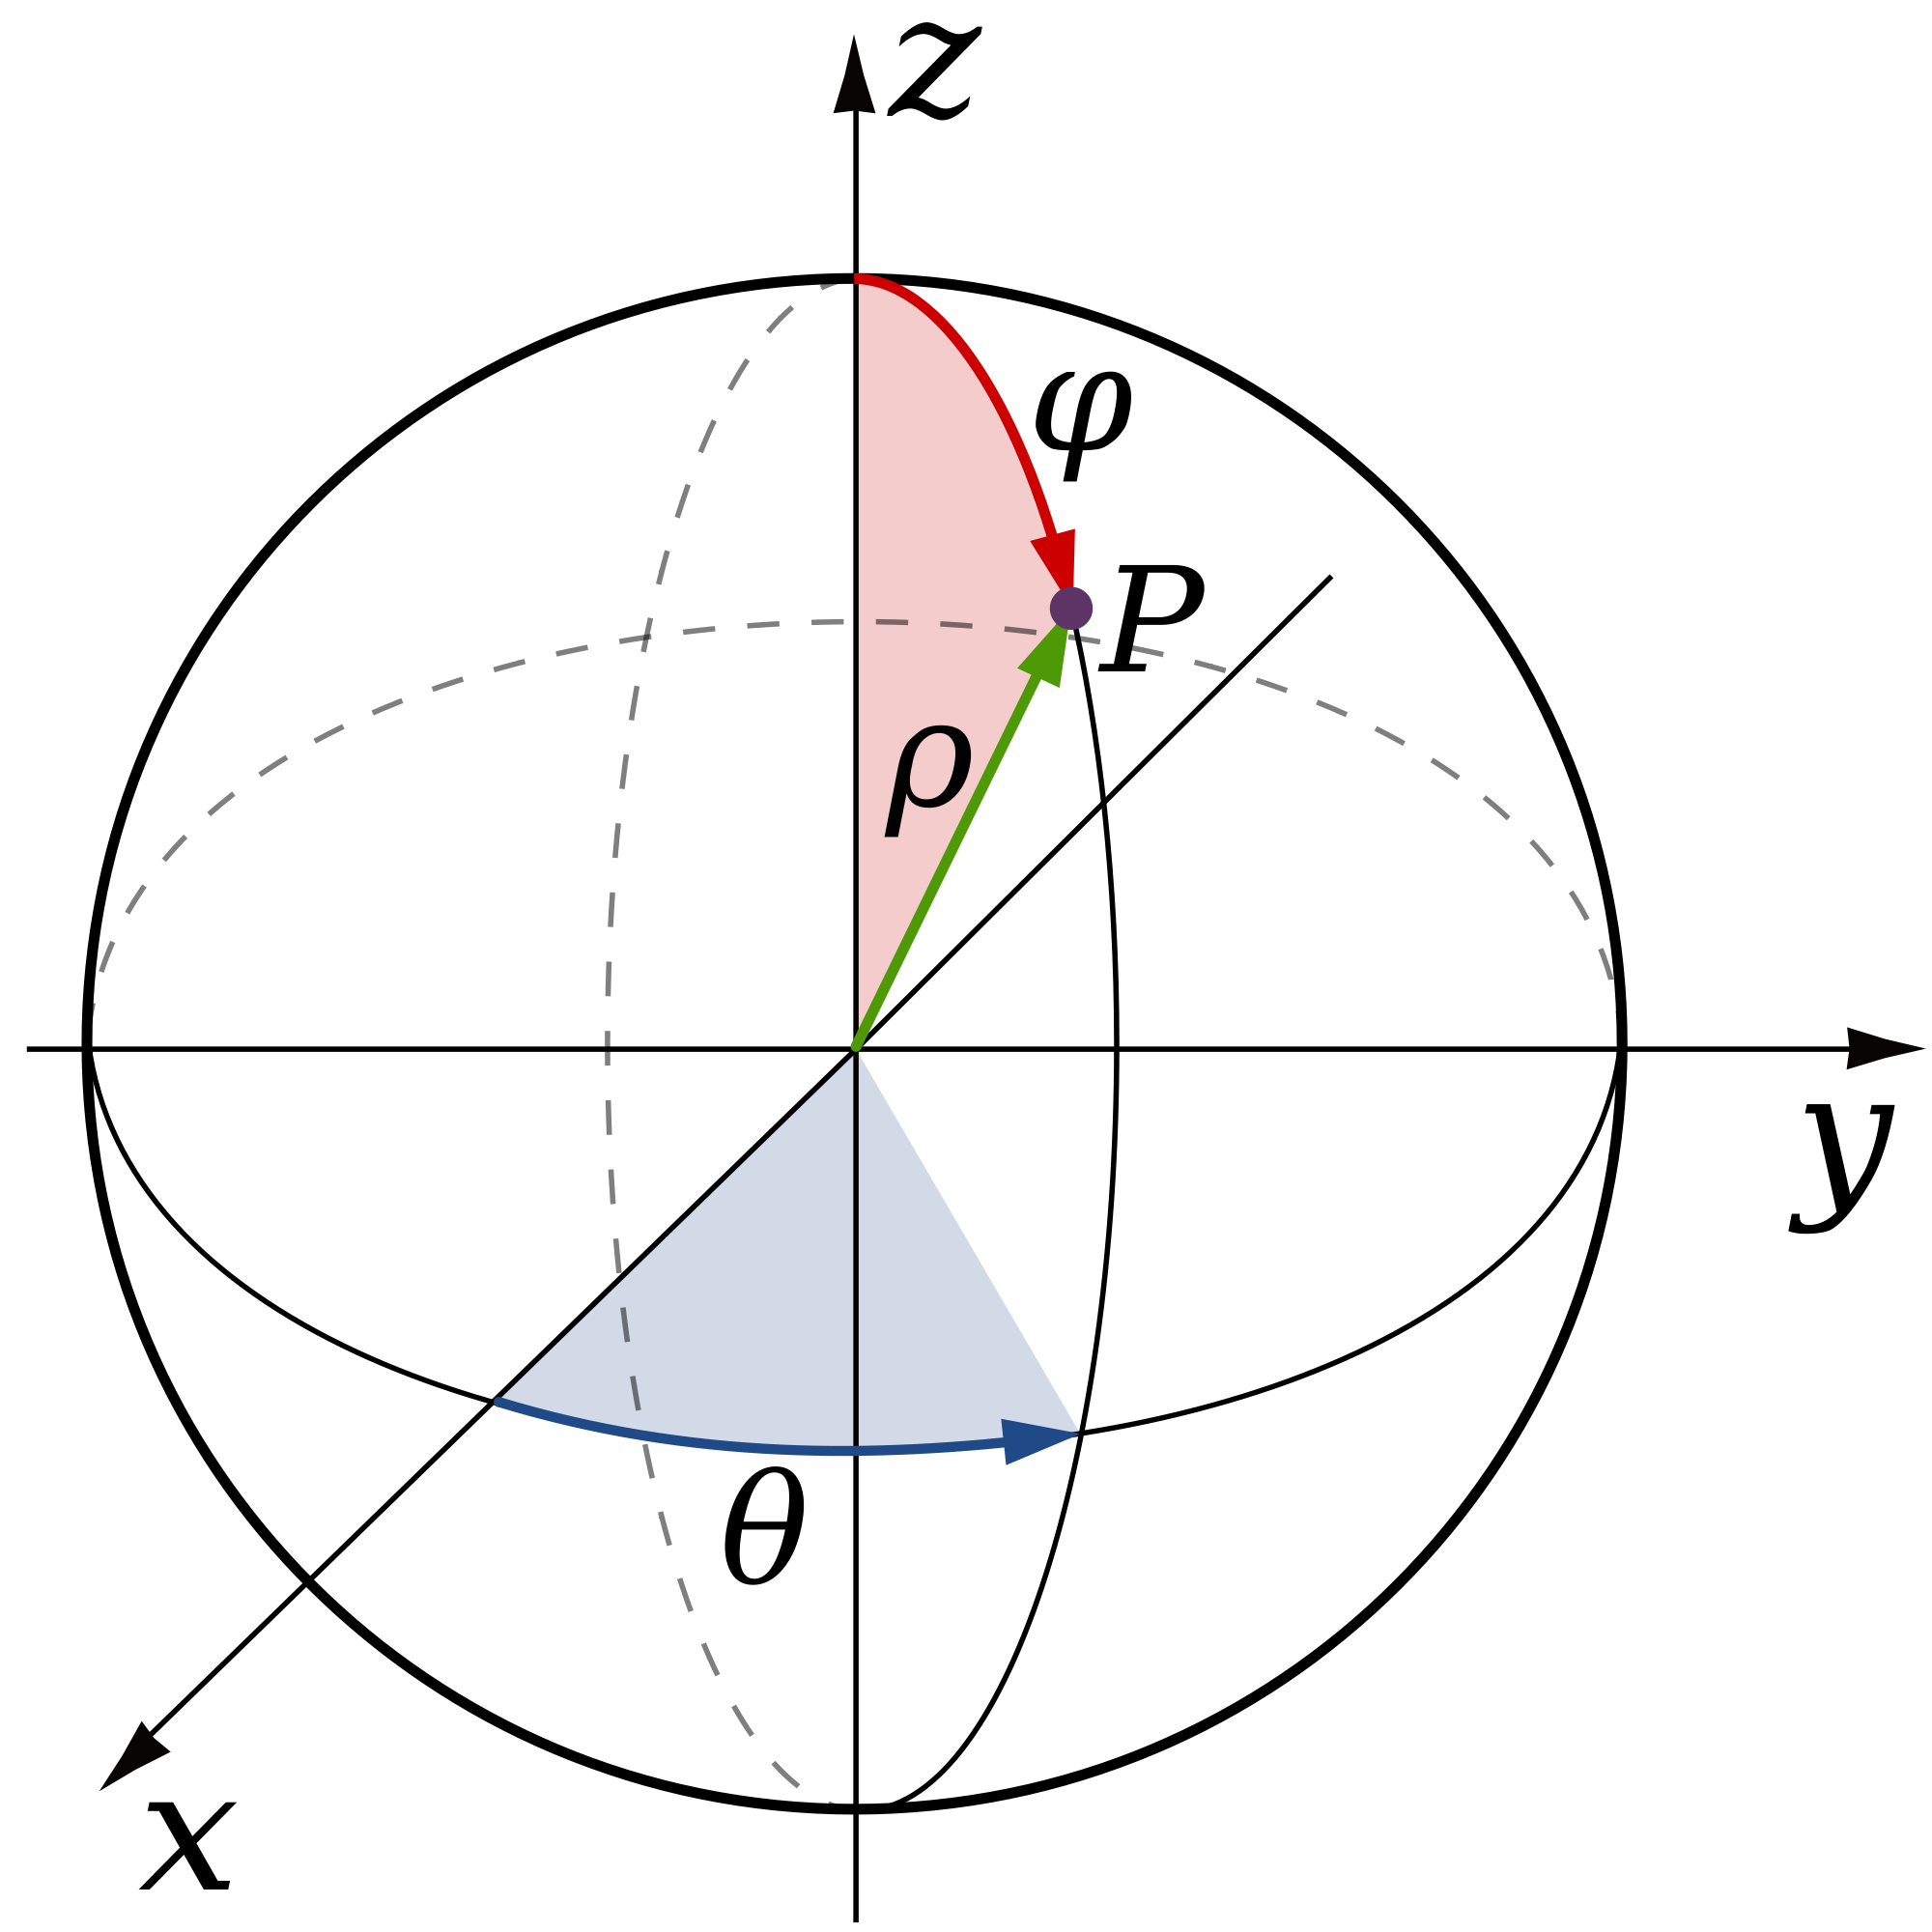
\includegraphics[width=0.5\linewidth]{znpVq.png}
\end{center}
Now, let $\theta \in (-\pi,\pi)$ and $\varphi \in (0,\pi)$. Some of you have taken $\varphi$ as the elevation angle, in this case it would be $\varphi \in (-\frac{\pi}{2},\frac{\pi}{2})$ and the function won't have the $-\frac{\pi}{2}$ for the Y part.

We use the function - 
\begin{align*}
    f(\theta,\varphi) &= \Bigg(tan\bigg(\frac{\theta}{2}\bigg),tan\bigg(\varphi - \frac{\pi}{2}\bigg)\Bigg)
\end{align*}
We know $tan(\theta)$ is a bijective function on the interval $(-\frac{\pi}{2},\frac{\pi}{2})$. You can draw the graph too [not necessary].

Now we realise that for all $\theta = \pi$, we won't be able to define $f$. And similarly, for all $\varphi = 0,$ and $\pi$, we won't be able to define $f$, and they will be left unmapped. For this, we first realise what do they correspond to - 
\begin{center}
    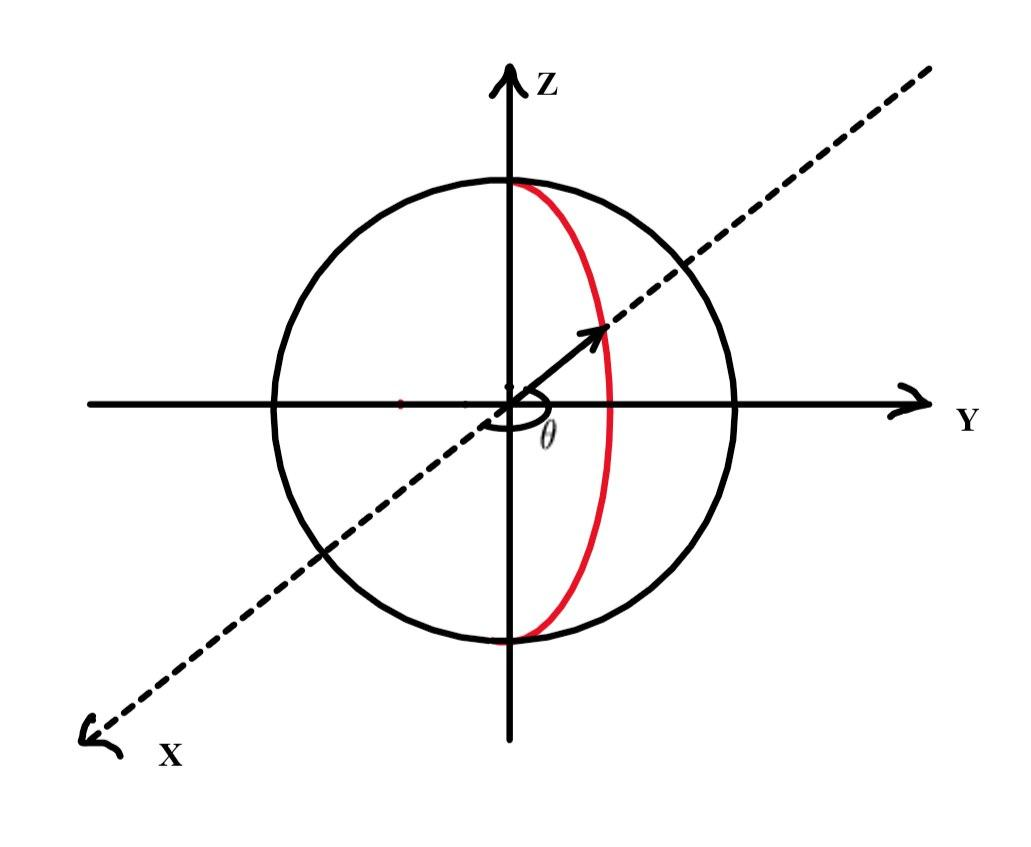
\includegraphics[width=0.7\linewidth]{photo_2020-10-31_16-28-07.jpg}
\end{center}
The red line above corresponds to all the points with $\theta = \pi$.
\begin{center}
    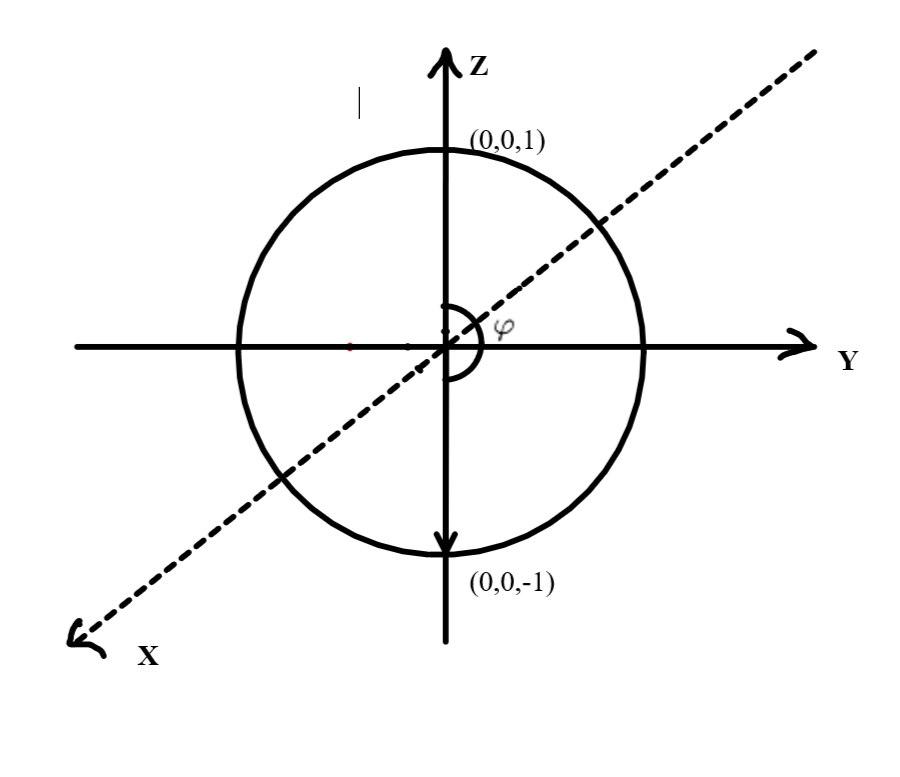
\includegraphics[width=0.7\linewidth]{photo_2020-10-31_16-32-03.jpg}
\end{center}
The point $(0,0,1)$ and $(0,0,-1)$ are the points with $\varphi = 0,$ and $\pi$ respectively.

Now we map the red arc to a line using the bijection $tan(\varphi - \frac{\pi}{2})$. (again, the poles will be unmapped). Name this line $l_1$.

Take any line in the plane, say, the X-axis. Name this line $l_2$.

We will construct a new line $l$ using $l_1$ and $l_2$. Let $P(m)$ denote the set of all points in any line $m$. Define $f:P(l_1) \cup P(l_2) \rightarrow P(l)$ as follows - 
\begin{align*}
f(x) &=
    \begin{cases}
     tan\bigg(\frac{tan^{-1}(x) -  \frac{\pi}{2}}{2}\bigg) \text{ if $x \in P(l_1)$}\\ 
     tan\bigg(\frac{tan^{-1}(x) + \frac{\pi}{2}}{2}\bigg) \text{ if $x \in P(l_2)$}\\
    \end{cases}
\end{align*}
We prove that $f$ is bijective mapping, notice that the first part maps all the points in $l_1$ to an interval $(-\frac{\pi}{2},0)$, and the second part maps all the points in $l_2$ to the interval $(0,\frac{\pi}{2})$ (before taking $tan$ on each).

 Here $(0,0)$ is not mapped. Thus the cardinality of $P(l) - (0,0)$ is same as $P(l_1) \cup P(l_2)$. We map $(0,0,-1)$ to this $(0,0)$.
 And thus the only point left unmapped is $(0,0,1)$  which does not change the cardinality as it is a finite set .

\\ \textbf{Method 3:}
\\ \textbf{Using a point source of light -} 
We can use a point source of light at the center of the sphere to render 2 planes as follows - 

\begin{center}
    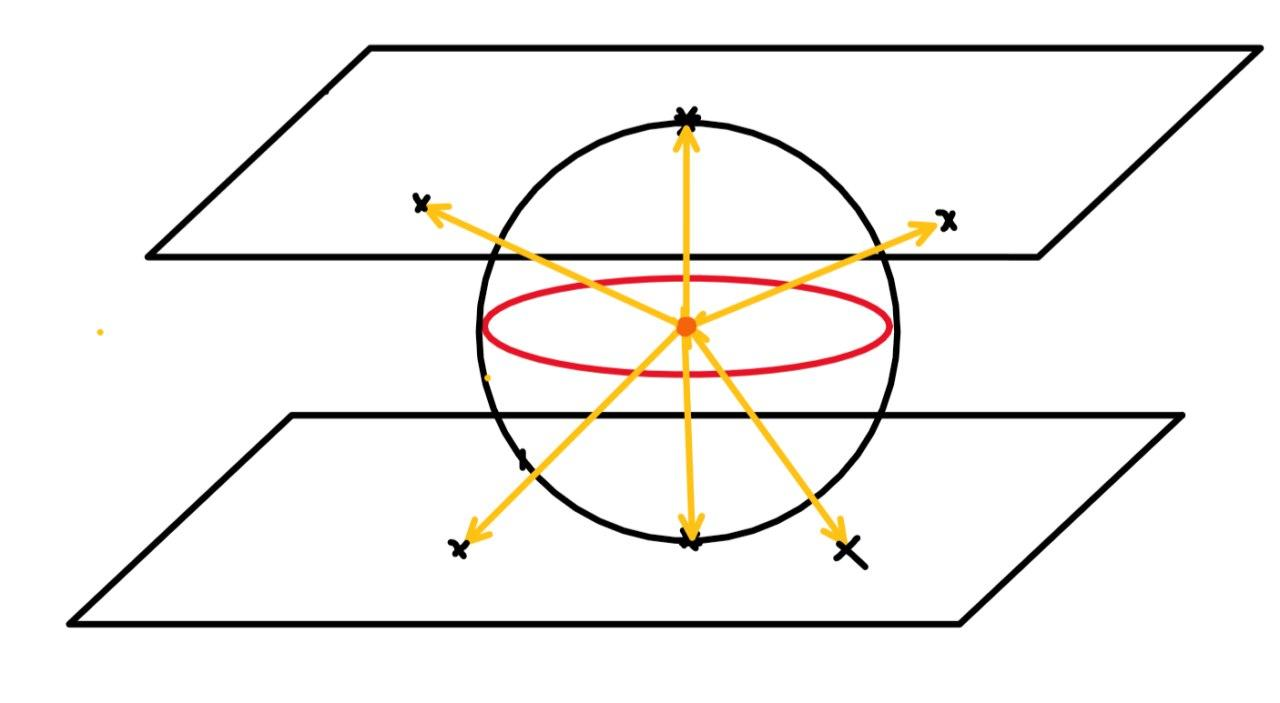
\includegraphics[width=0.7\linewidth]{photo_2020-11-02_11-44-00.jpg}
\end{center}
Each lattitude on the sphere will be mapped to a circle on the plane, and that the poles will be mapped to the tangent point of the 2 planes to the sphere. To prove this is bijection is easy, as for each point on the plane, you will just have one light ray from the source at origin to itself. And for each point on the plane, you will have a ray coming from center of sphere to itself.

Now you will notice that the \textbf{equator (red)} is still left unmapped. And that there are 2 planes instead of one. Now we first map the 2 planes to one plane - 

Call the two planes $\Gamma_1$ and $\Gamma_2$. Let $Q(m)$ denote the set of all points in any line $m$. Construct a new plane $\Gamma$ from $\Gamma_1$ and $\Gamma_2$ such that 
\begin{align*}
f(x,y) &=
    \begin{cases}
     \bigg(tan\bigg(\frac{tan^{-1}(x) -  \frac{\pi}{2}}{2}\bigg),tan\bigg(tan^{-1}(y)\bigg)\bigg) \text{ if $(x,y) \in Q(\Gamma_1)$}\\ 
     \bigg(tan\bigg(\frac{tan^{-1}(x) + \frac{\pi}{2}}{2}\bigg),tan\bigg(tan^{-1}(y))\bigg)\bigg) \text{ if $(x,y) \in Q(\Gamma_2)$}\\
    \end{cases}
\end{align*}
Notice that the points on the X axis will be left unmapped. Here we map our equator to a line using the $tan(\frac{\theta}{2})$ argument discussed in the Tut. Thus, no point is left unmapped here.
\paragraph*{Problem 7}
There are 2 ways mainly to prove this - 
\begin{enumerate}
    \item Prove and use the property that $f$ is injective $\iff$ $f$ has a left inverse. Thus you get 
    \begin{align*}
         & g \circ f (x_1) = g \circ f(x_2)
        \\ & \implies f(x_1) = f(x_2) & \text{\{Since $g$ is injective\}}
        \\ & \implies x_1 = x_2 & \text{\{Since $f$ is injective\}}
     \end{align*}
     We have cut your marks if you directly stated without the proof. We expect you to do the proof since it was done in the Tutorial.
    \item Let $f:R \rightarrow T$ and $g:T \rightarrow U$ have left inverses $\phi:T \rightarrow R$ and $\gamma: U \rightarrow T$. We have  $\gamma \circ g = I_T$ and $\phi \circ f = I_R$.
    \begin{align*}
        & ( \gamma \circ \phi ) \circ (g \circ f) 
        \\ &= (\phi  \circ (\gamma  \circ g)) \circ f) & \text{ \{Since $\circ$ composition is associative\}}
        \\ &= (\phi \circ I_T) \circ f & \text{ \{By definition\}}
        \\ &= \phi \circ f & \text{ \{Idempotency, $f \circ I_{dom(f)} = f$\}}
        \\ &= I_R & \text{ \{By definition\}}
    \end{align*}
    Thus the inverse is $\gamma \circ \phi$.
\end{enumerate}


\paragraph*{Problem 8}
We construct a mapping $f:S \rightarrow \mathbb{N}$ where $S$ is the set of positive integers(natural numbers) divisible by 5.
\begin{align*}
    f(n) = \frac{n}{5}
\end{align*}
\begin{enumerate}
    \item \textbf{One-One}
    \\ \begin{align*}
        & f(n_1) = f(n_2)
        \\  &\implies \frac{n_1}{5} = \frac{n_2}{5}
        \\ & \implies n_1 = n_2
    \end{align*}
    \item \textbf{Onto}
    We have \begin{align*}
        \forall p \in \mathbb{N}, f(5p) = \frac{5p}{5} = p
    \end{align*}
    Thus pre-image exists for all elements.
\end{enumerate}
Some of you have showed the mapping from  $\mathbb{Z}$ to $\mathbb{N}$, and used the theorem that every subset of a countable set is countable. If you have proved the theorem, then we have given you marks. Note that $S$ is a subset of $\mathbb{N}$ itself and you can use the theorem directly (after proving it) instead of using  $\mathbb{Z}$.
\end{document}

